\documentclass[tikz,border=8pt]{standalone}
% Shared look for every TikZ diagram. Load with \input{../../tools/tikz-style.tex}
\usepackage[T1]{fontenc}
\usepackage{lmodern}
\renewcommand{\sfdefault}{lmr}  % diagrams use the same serif as the text
\usetikzlibrary{arrows.meta, positioning, shapes.geometric, calc, fit, backgrounds}
\definecolor{cblue}{HTML}{4C78A8}
\definecolor{corange}{HTML}{F58518}
\definecolor{cgreen}{HTML}{54A24B}
\definecolor{cred}{HTML}{E45756}
\definecolor{cpurple}{HTML}{B279A2}
\definecolor{cgrey}{HTML}{6B6B6B}
\tikzset{
  every picture/.style={font=\sffamily, line width=1.2pt},
  box/.style={draw=#1, fill=#1!12, rounded corners=4pt, align=center, inner sep=7pt, minimum height=1.1cm},
  box/.default=cgrey,
  arrow/.style={-{Stealth[length=3mm]}, draw=cgrey, line width=1.4pt},
  title/.style={font=\sffamily\bfseries\Large},
  note/.style={font=\sffamily\small, text=cgrey, align=center},
}
\AtBeginDocument{\hyphenpenalty=10000 \exhyphenpenalty=10000}

\begin{document}
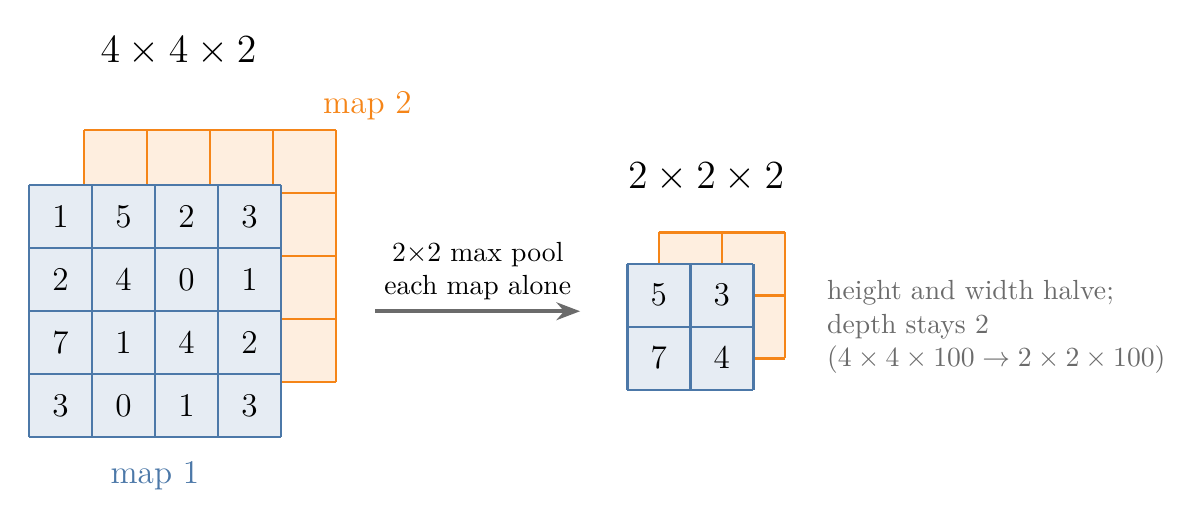
\begin{tikzpicture}
  % a square map of n cells, side s, at (x,y), colour c, optional numbers
  \newcommand{\grid}[5]{% x y n s colour
    \fill[#5!14] (#1,#2) rectangle ++(#3*#4,#3*#4);
    \draw[#5, line width=0.9pt, step=#4, shift={(#1,#2)}] (0,0) grid (#3*#4,#3*#4);}
  % input volume 4x4x2: back map then front map
  \grid{0.7}{0.7}{4}{0.8}{corange}
  \grid{0}{0}{4}{0.8}{cblue}
  \foreach \v [count=\i from 0] in {1,5,2,3,2,4,0,1,7,1,4,2,3,0,1,3}{
    \pgfmathtruncatemacro{\r}{\i/4}\pgfmathtruncatemacro{\c}{mod(\i,4)}
    \node[font=\sffamily\large] at (0.4+0.8*\c, 2.8-0.8*\r) {\v};}
  \node[font=\sffamily\large, text=corange] at (4.3,4.2) {map 2};
  \node[font=\sffamily\large, text=cblue] at (1.6,-0.5) {map 1};
  \node[title] at (1.9,4.9) {$4\times4\times2$};
  \draw[arrow] (4.4,1.6) -- (7.0,1.6) node[midway, above, align=center] {2$\times$2 max pool\\each map alone};
  % output 2x2x2
  \grid{8.0}{1.0}{2}{0.8}{corange}
  \grid{7.6}{0.6}{2}{0.8}{cblue}
  \foreach \v [count=\i from 0] in {5,3,7,4}{
    \pgfmathtruncatemacro{\r}{\i/2}\pgfmathtruncatemacro{\c}{mod(\i,2)}
    \node[font=\sffamily\large] at (8.0+0.8*\c, 1.8-0.8*\r) {\v};}
  \node[title] at (8.6,3.3) {$2\times2\times2$};
  \node[note, font=\sffamily\normalsize, align=left, anchor=west] at (10.0,1.4) {height and width halve;\\depth stays 2\\($4\times4\times100 \rightarrow 2\times2\times100$)};
\end{tikzpicture}
\end{document}
